\begin{figure}[H]
    \centering
    \begin{subfigure}{0.075\textwidth} \includegraphics[width=\linewidth]{data/heat_entropy/0.png}  \caption{} \end{subfigure}
    
    \begin{subfigure}{0.19\textwidth} 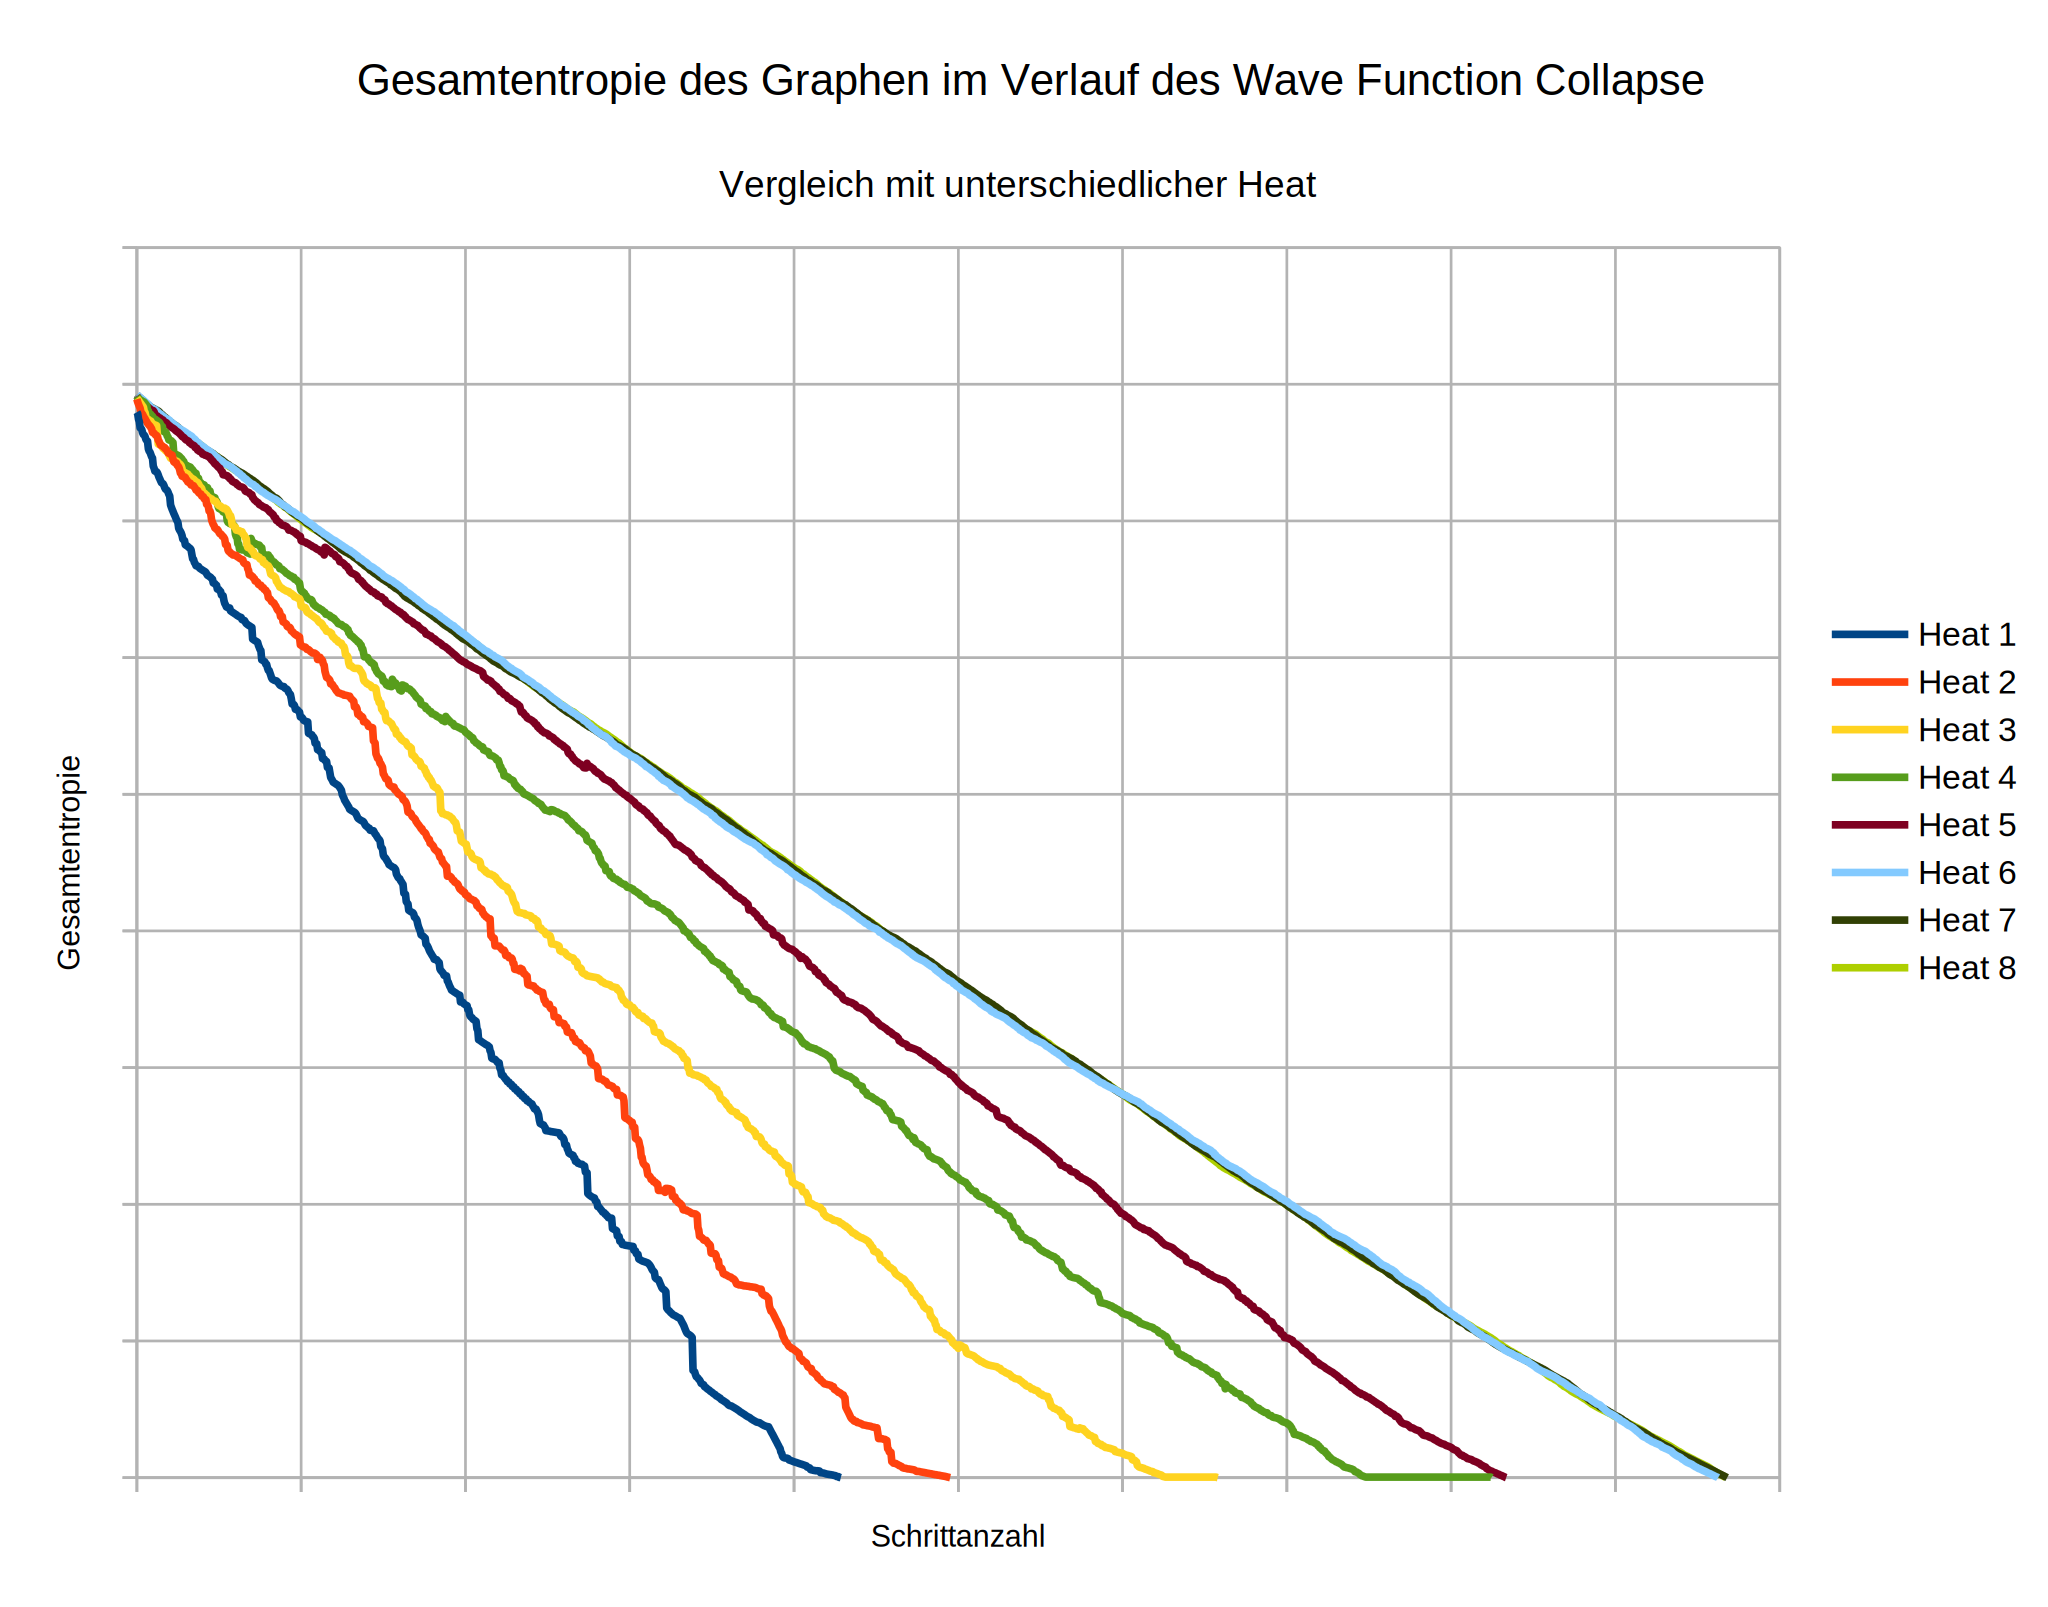
\includegraphics[width=\linewidth]{data/heat_entropy/1.png}  \caption{$H=1$ $S=1$} \end{subfigure}
    \hspace{1em}
    \begin{subfigure}{0.19\textwidth} \includegraphics[width=\linewidth]{data/heat_entropy/2.png}  \caption{$H=1$ $S=5$} \end{subfigure}
    \hspace{3em}
    \begin{subfigure}{0.19\textwidth} \includegraphics[width=\linewidth]{data/heat_entropy/3.png}  \caption{$H=2$ $S=1$} \end{subfigure}
    \hspace{1em}
    \begin{subfigure}{0.19\textwidth} \includegraphics[width=\linewidth]{data/heat_entropy/4.png}  \caption{$H=2$ $S=5$} \end{subfigure}

    \begin{subfigure}{0.19\textwidth} \includegraphics[width=\linewidth]{data/heat_entropy/5.png}  \caption{$H=3$ $S=1$} \end{subfigure}
    \hspace{1em}
    \begin{subfigure}{0.19\textwidth} \includegraphics[width=\linewidth]{data/heat_entropy/6.png}  \caption{$H=3$ $S=5$} \end{subfigure}
    \hspace{3em}
    \begin{subfigure}{0.19\textwidth} \includegraphics[width=\linewidth]{data/heat_entropy/7.png}  \caption{$H=4$ $S=1$} \end{subfigure}
    \hspace{1em}
    \begin{subfigure}{0.19\textwidth} \includegraphics[width=\linewidth]{data/heat_entropy/8.png}  \caption{$H=4$ $S=5$} \end{subfigure}

    \begin{subfigure}{0.19\textwidth} \includegraphics[width=\linewidth]{data/heat_entropy/9.png}  \caption{$H=5$ $S=1$} \end{subfigure}
    \hspace{1em}
    \begin{subfigure}{0.19\textwidth} \includegraphics[width=\linewidth]{data/heat_entropy/10.png} \caption{$H=5$ $S=5$} \end{subfigure}
    \hspace{3em}
    \begin{subfigure}{0.19\textwidth} \includegraphics[width=\linewidth]{data/heat_entropy/11.png} \caption{$H=6$ $S=1$} \end{subfigure}
    \hspace{1em}
    \begin{subfigure}{0.19\textwidth} \includegraphics[width=\linewidth]{data/heat_entropy/12.png} \caption{$H=6$ $S=5$} \end{subfigure}

    \begin{subfigure}{0.19\textwidth} \includegraphics[width=\linewidth]{data/heat_entropy/13.png} \caption{$H=7$ $S=1$} \end{subfigure}
    \hspace{1em}
    \begin{subfigure}{0.19\textwidth} \includegraphics[width=\linewidth]{data/heat_entropy/14.png} \caption{$H=7$ $S=5$} \end{subfigure}
    \hspace{3em}
    \begin{subfigure}{0.19\textwidth} \includegraphics[width=\linewidth]{data/heat_entropy/15.png} \caption{$H=8$ $S=1$} \end{subfigure}
    \hspace{1em}
    \begin{subfigure}{0.19\textwidth} \includegraphics[width=\linewidth]{data/heat_entropy/16.png} \caption{$H=8$ $S=5$} \end{subfigure}
    
    \caption{
        Die Entropie der Zellen nach jeweils einem und fünf Schritten des Algorithmus mit unterschiedlicher Heat. (a) zeigt das Beispiel. Für (b-q) ist $H$ die Heat und $S$ die Anzahl der Schritte. Rot entspricht hoher Entropie, kollabierte Zellen zeigen ihren finalen Zustand(hier Grau oder Schwarz).
    }
    \label{fig:heat_entropy}
\end{figure}